\chapter{Практические результаты}
\section{Наибольшая общая Абелева подстрока}
\subsection{Случай бинарного алфавита}

Первое, что хочется сделать~--- посмотреть, как же ведет себя на практике матожидание наибольшей общей Абелевой подстроки двух случайных бинарных строк. 

Я выполнил на своем ноутбуке (на кластере канеш) $10^4$ запусков поиска НОАП для различных $n$ до $10^4$. Такого количества запусков оказалось достаточно, чтобы среднее значение примерно сошлось (мб даже стоит попруфать, дисперсию там какую-нить оценить). Полученный результат можно увидеть на рисунке 1.

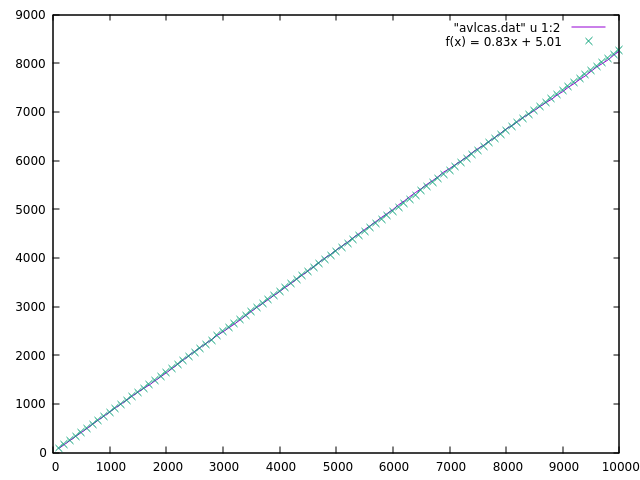
\includegraphics{pics/avlcas.png}

Видно, что функция ведет себя очень точно как прямая $y=0.83x$, что подтверждает линейные оценки как сверху, так и снизу.

Вычислить точное значение этого коэффициента, или строгие оценки на него сверху и снизу остается открытой задачей. 

%\subsection{Общий случай}
%Пусто? Ну я канеш могу закодить то что я придумал но не оч хочется(((

\section{Количество Абелевых подквадратов}

Реализованный алгоритм решения 3SUM работает очень медленно

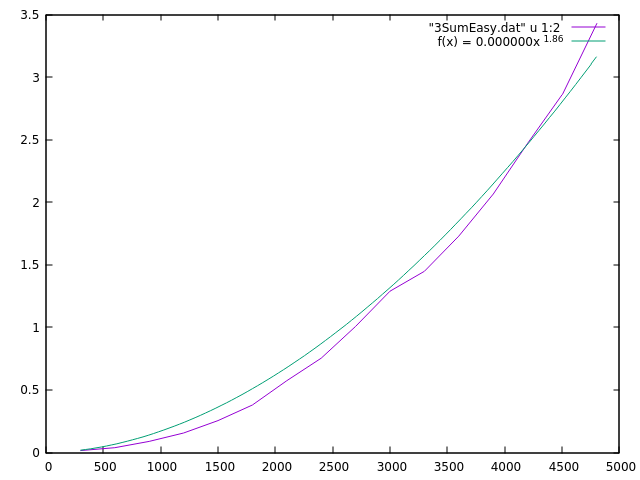
\includegraphics[scale=1]{pics/4.png}

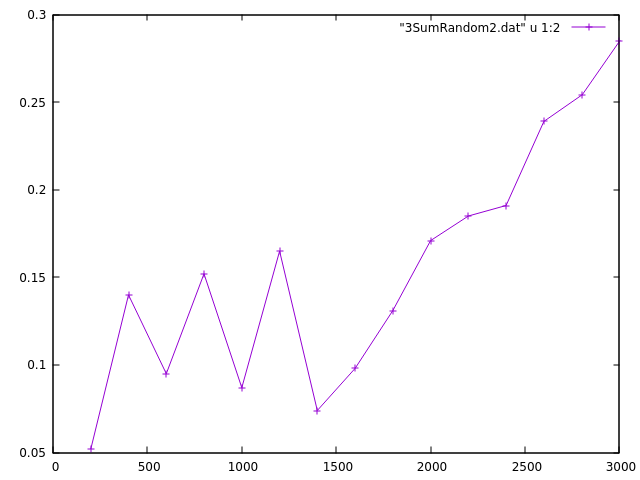
\includegraphics[scale=1]{pics/5.png}